% Created by tikzDevice version 0.12.6 on 2025-08-19 18:47:28
% !TEX encoding = UTF-8 Unicode
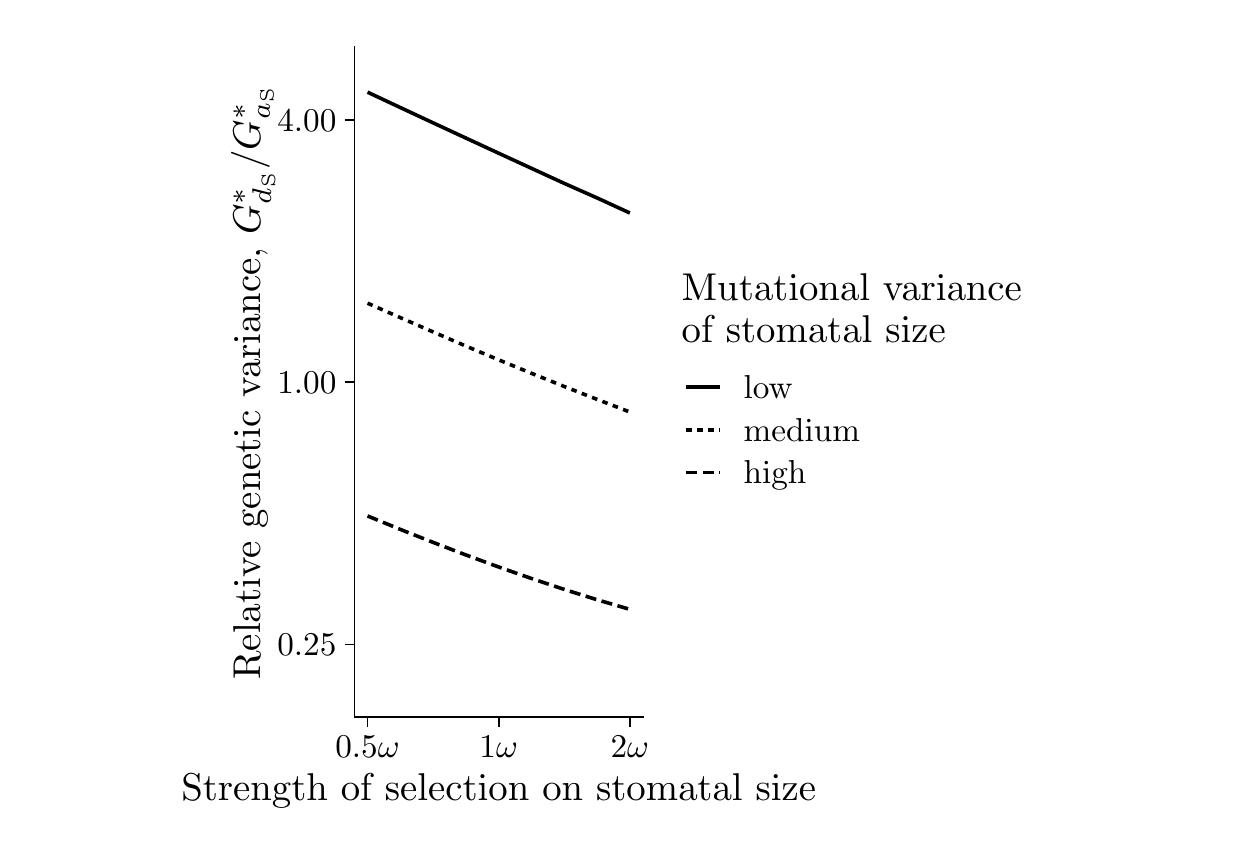
\begin{tikzpicture}[x=1pt,y=1pt]
\definecolor{fillColor}{RGB}{255,255,255}
\path[use as bounding box,fill=fillColor,fill opacity=0.00] (0,0) rectangle (433.62,289.08);
\begin{scope}
\path[clip] (118.07, 39.96) rectangle (222.34,282.08);
\definecolor{drawColor}{RGB}{0,0,0}

\path[draw=drawColor,line width= 1.3pt,line join=round] (122.81,265.77) --
	(134.66,260.21) --
	(146.51,254.68) --
	(158.36,249.18) --
	(170.21,243.70) --
	(182.06,238.24) --
	(193.91,232.80) --
	(205.76,227.55) --
	(217.60,222.11);

\path[draw=drawColor,line width= 1.3pt,dash pattern=on 2pt off 2pt ,line join=round] (122.81,189.52) --
	(134.66,184.30) --
	(146.51,179.13) --
	(158.36,174.02) --
	(170.21,169.04) --
	(182.06,164.18) --
	(193.91,159.41) --
	(205.76,154.76) --
	(217.60,150.19);

\path[draw=drawColor,line width= 1.3pt,dash pattern=on 4pt off 2pt ,line join=round] (122.81,112.64) --
	(134.66,107.78) --
	(146.51,103.08) --
	(158.36, 98.54) --
	(170.21, 94.19) --
	(182.06, 90.03) --
	(193.91, 86.08) --
	(205.76, 82.36) --
	(217.60, 78.89);
\end{scope}
\begin{scope}
\path[clip] (  0.00,  0.00) rectangle (433.62,289.08);
\definecolor{drawColor}{RGB}{0,0,0}

\path[draw=drawColor,line width= 0.6pt,line join=round,line cap=rect] (118.07, 39.96) --
	(118.07,282.08);
\end{scope}
\begin{scope}
\path[clip] (  0.00,  0.00) rectangle (433.62,289.08);
\definecolor{drawColor}{RGB}{0,0,0}

\node[text=drawColor,anchor=base east,inner sep=0pt, outer sep=0pt, scale=  1.20] at (111.57, 62.09) {0.25};

\node[text=drawColor,anchor=base east,inner sep=0pt, outer sep=0pt, scale=  1.20] at (111.57,156.89) {1.00};

\node[text=drawColor,anchor=base east,inner sep=0pt, outer sep=0pt, scale=  1.20] at (111.57,251.68) {4.00};
\end{scope}
\begin{scope}
\path[clip] (  0.00,  0.00) rectangle (433.62,289.08);
\definecolor{drawColor}{RGB}{0,0,0}

\path[draw=drawColor,line width= 0.6pt,line join=round] (114.57, 66.23) --
	(118.07, 66.23);

\path[draw=drawColor,line width= 0.6pt,line join=round] (114.57,161.02) --
	(118.07,161.02);

\path[draw=drawColor,line width= 0.6pt,line join=round] (114.57,255.82) --
	(118.07,255.82);
\end{scope}
\begin{scope}
\path[clip] (  0.00,  0.00) rectangle (433.62,289.08);
\definecolor{drawColor}{RGB}{0,0,0}

\path[draw=drawColor,line width= 0.6pt,line join=round,line cap=rect] (118.07, 39.96) --
	(222.34, 39.96);
\end{scope}
\begin{scope}
\path[clip] (  0.00,  0.00) rectangle (433.62,289.08);
\definecolor{drawColor}{RGB}{0,0,0}

\path[draw=drawColor,line width= 0.6pt,line join=round] (122.81, 36.46) --
	(122.81, 39.96);

\path[draw=drawColor,line width= 0.6pt,line join=round] (170.21, 36.46) --
	(170.21, 39.96);

\path[draw=drawColor,line width= 0.6pt,line join=round] (217.60, 36.46) --
	(217.60, 39.96);
\end{scope}
\begin{scope}
\path[clip] (  0.00,  0.00) rectangle (433.62,289.08);
\definecolor{drawColor}{RGB}{0,0,0}

\node[text=drawColor,anchor=base,inner sep=0pt, outer sep=0pt, scale=  1.20] at (122.81, 25.20) {$0.5\omega$};

\node[text=drawColor,anchor=base,inner sep=0pt, outer sep=0pt, scale=  1.20] at (170.21, 25.20) {$1\omega$};

\node[text=drawColor,anchor=base,inner sep=0pt, outer sep=0pt, scale=  1.20] at (217.60, 25.20) {$2\omega$};
\end{scope}
\begin{scope}
\path[clip] (  0.00,  0.00) rectangle (433.62,289.08);
\definecolor{drawColor}{RGB}{0,0,0}

\node[text=drawColor,anchor=base,inner sep=0pt, outer sep=0pt, scale=  1.40] at (170.21,  9.72) {Strength of selection on stomatal size};
\end{scope}
\begin{scope}
\path[clip] (  0.00,  0.00) rectangle (433.62,289.08);
\definecolor{drawColor}{RGB}{0,0,0}

\node[text=drawColor,rotate= 90.00,anchor=base,inner sep=0pt, outer sep=0pt, scale=  1.40] at ( 84.02,161.02) {Relative genetic variance, $G^*_{d_\mathrm{S}} / G^*_{a_\mathrm{S}}$};
\end{scope}
\begin{scope}
\path[clip] (  0.00,  0.00) rectangle (433.62,289.08);
\definecolor{drawColor}{RGB}{0,0,0}

\node[text=drawColor,anchor=base west,inner sep=0pt, outer sep=0pt, scale=  1.40] at (236.34,190.36) {Mutational variance};

\node[text=drawColor,anchor=base west,inner sep=0pt, outer sep=0pt, scale=  1.40] at (236.34,175.24) {of stomatal size};
\end{scope}
\begin{scope}
\path[clip] (  0.00,  0.00) rectangle (433.62,289.08);
\definecolor{drawColor}{RGB}{0,0,0}

\path[draw=drawColor,line width= 1.3pt,line join=round] (237.88,159.18) -- (250.20,159.18);
\end{scope}
\begin{scope}
\path[clip] (  0.00,  0.00) rectangle (433.62,289.08);
\definecolor{drawColor}{RGB}{0,0,0}

\path[draw=drawColor,line width= 1.3pt,dash pattern=on 2pt off 2pt ,line join=round] (237.88,143.78) -- (250.20,143.78);
\end{scope}
\begin{scope}
\path[clip] (  0.00,  0.00) rectangle (433.62,289.08);
\definecolor{drawColor}{RGB}{0,0,0}

\path[draw=drawColor,line width= 1.3pt,dash pattern=on 4pt off 2pt ,line join=round] (237.88,128.38) -- (250.20,128.38);
\end{scope}
\begin{scope}
\path[clip] (  0.00,  0.00) rectangle (433.62,289.08);
\definecolor{drawColor}{RGB}{0,0,0}

\node[text=drawColor,anchor=base west,inner sep=0pt, outer sep=0pt, scale=  1.20] at (258.74,155.05) {low};
\end{scope}
\begin{scope}
\path[clip] (  0.00,  0.00) rectangle (433.62,289.08);
\definecolor{drawColor}{RGB}{0,0,0}

\node[text=drawColor,anchor=base west,inner sep=0pt, outer sep=0pt, scale=  1.20] at (258.74,139.65) {medium};
\end{scope}
\begin{scope}
\path[clip] (  0.00,  0.00) rectangle (433.62,289.08);
\definecolor{drawColor}{RGB}{0,0,0}

\node[text=drawColor,anchor=base west,inner sep=0pt, outer sep=0pt, scale=  1.20] at (258.74,124.25) {high};
\end{scope}
\end{tikzpicture}
